\chapter{Winters \& D'Asaro (1996): $K_T$, $J_q^t$ from $χ$}

\section{Usage}

\texttt{main\_driver} options:
\begin{itemize}
\item
  \texttt{pflag.master.winters\_dasaro} : switch on (1) or off (0)
\item
  \texttt{pflag.master.wda\_dt} : (seconds) length of time chunk that is processed at a time. Default is 60 seconds which works OK in the top 30m or so. For deeper χpods you can go longer (3 minutes?)
\end{itemize}

\texttt{combine\_turbulence} options:
\begin{itemize}
\item
  \texttt{CP.wda\_Tz\_sign} : (\texttt{'m'} or \texttt{'i'}) - gradient time series used to assign sign to heat flux.
\end{itemize}


The output \texttt{Turb.mat} file will contain \texttt{wda} substructure under each estimate i.e. for estimate \texttt{mm1} the fields \texttt{mm1.wda.Jq, mm1.wda.Kt} are estimates computed using the sorted temperature field. \emph{These are different from \texttt{mm1.Jq, mm1.Kt} which are set using the old way of doing things i.e. dividing by mooring gradient in this case.}

Because we are using the sorted $T_z$ field, there is no reason to mask using \texttt{min\_dTdz}.
All other masking is applied.

\section{Theory}
\newcommand{\Tbins}{T_\text{bins}}
\newcommand{\zs}{z_{*}}

Osborn \& Cox:
\begin{equation}
  J_q^t \sim \frac{\langle χ \rangle}{⟨\pp Tz⟩}
\end{equation}
These angle brackets are interpreted as a time average for χpods and a depth-bin average for profilers like Chameleon.

The Osborn \& Cox formulation is not well behaved when stratification is low.
It gets worse in places with large salinity influence: large enough that $T_z < 0$ some of the time.
When $T_z$ crosses through zero, the estimates of $K_T, J_Q^t$ blow up.
In these cases, getting ``reasonable'' values for $K_T$ and $J_q^t$ requires masking out estimates when $T_z$ is less than some ill-defined threshold.

Winters \& D'Asaro derive the continuous form:
\begin{equation}
  J_q^t =  \dd{z^*}{T} \langle χ \rangle_{z^*}
\end{equation}

$z^*$ being the ``reference'' state — usually a fully sorted 3D scalar field.
In practice, we approximate this by Thorpe sorting single vertical profiles.
The angle brackets represent averaging in ``isoscalar'' (isothermal) space.

The Winters \& D'Asaro formulation has the advantage that it can be well-defined for low gradients — by thinking about distances between isoscalar surfaces.
The idea is that the averaging occurs in a volume between two isothermal surfaces.
The required gradient is then the average spacing between these two surfaces.
Doing this requires treating the χpod as a profiler, being pumped by surface waves.
We can keep track of the isotherms seen by the χpod in a chunk of data; and estimate the average distance between those isotherms as the χpod is pumped up and down.
For dense enough sampling this average distance should ideally converge to the distance between the isotherms in the fully sorted field (this being the necessary gradient).
Note that the χpod densely samples approximately 1-2 metres of the water column.

Why is the gradient of the (full 3D) sorted field the right gradient to use?
\begin{itemize}
  \item Mixing acts to change the background potential energy of the fluid --- the BPE is determined by computing the PE of the 3D-sorted density field.
  \item We want to infer the heat flux that goes into changing this BPE i.e. a sensible definition of heat flux is that which changes BPE by a given amount.
  \item The way to do this is to locate our $χ$ observations in the \emph{sorted reference state} and then compute heat flux --- the appropriate gradient being that of the sorted state.
  \end{itemize}
In practice, we approximate the gradient of the full 3D sorted state by differencing mooring CTDs, fitting a straight line to 50Hz temperature measurements (internal estimate) or sorting 1D profiles (as we do here).

An objection is that we know $T$ at \SI{100}{Hz} and $χ$ at \SI{1}{Hz}; and we want to sort $T$ at the highest possible frequency.
Consider however the discrete form of $J_q^t$ defined in \cite{Winters1996}.
Let $A_S$ is the surface-area of an extremely warped (stirred) temperature surface $S$ and $A$ be the area of that surface when it is flattened out so that $g$ is normal to it (Figure \ref{fig:wda-temp-surf}).
$J_q^t$ is the diffusive flux normal to the warped surface $S$ i.e. $κ∇T⋅\hat{n}$ integrated over $S$ — $κ$ is molecular diffusivity and $∇T⋅\hat{n} = \abs{∇T} ≈ ΔT/Δn$.
\begin{align}
  A J_q^t &= κ \int_S ∇T⋅\hat{n} \dr S \\
  J_q^t &= \frac{1}{A} \int_S κ \abs{∇T} \frac{ΔT}{Δn} \frac{Δn}{ΔT} \frac{Δ\zs}{Δ\zs} \dr S\\
        &= \frac{1}{AΔ\zs} \int_S χ \frac{Δ\zs}{ΔT} Δn \dr S
\end{align}

$Δ\zs/ΔT$, a property of the sorted background state, is independent of the instantaneous shape of the isothermal surface $S$. So we can write
\begin{equation}
 J_q^t = \frac{Δ\zs}{ΔT} \frac{1}{AΔ\zs} \int_S χ Δn \dr S = \frac{Δ\zs}{ΔT} \frac{1}{ΔV} \int_{ΔV} χ \dr V,
\end{equation}
since $\zs$ is \emph{defined} such that
\begin{equation}
   AΔ\zs = \int_S Δn \dr S = ΔV = \text{volume of fluid between surfaces separated by} Δ\zs \text{ or } ΔT.
\end{equation}
$J_q^t$ is the product of $Δ\zs/ΔT$ and the \emph{volume-averaged} $χ$ between those two surfaces separated by $ΔT, Δ\zs$.
In low stratification, estimating the spacing requires high-resolution temperature measurements but that is exactly what the χpod does.

\begin{figure}[htbp]
  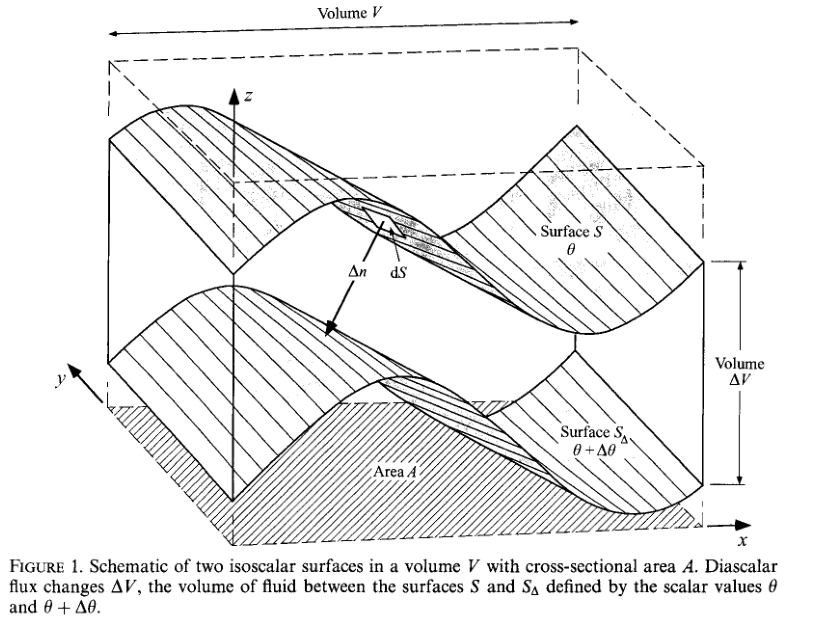
\includegraphics[width=0.9\textwidth]{figs/winters-dasaro-temp-surfaces.png}
  \caption{Figure reproduced from \cite{Winters1996}.}
  \label{fig:wda-temp-surf}
\end{figure}

\section{Algorithm}
Consider a 1 minute (configurable parameter \texttt{pflag.master.wda\_dt}) chunk of data.
\begin{itemize}
\item
  Once $χ$ has been estimated, we have $χ ≡ χ(t) ≡ χ(T_1)$, $T_1$ is the 1-second averaged temperature time series.

\item
  We can divide the temperature time series into $N$ quantiles, bin the $χ$ estimates in these temperature bins and then average them to get $\langle  χ \rangle ≡ χ(Δ\Tbins)$. $Δ\Tbins$ represents the bins between bin edges $\Tbins$. This is what \cite{Winters1996} call ``isoscalar averaging'' --- every $χ$ estimate made between 2 isothermal surfaces is averaged together.

\item
  Next, we need to determine the average distance between the isothermal surfaces $\Tbins$.
  \begin{itemize}
  \item
    Determine the start and end of ``up-'' and ``down-''casts using the intergrated accelerometer. Discard those that aren't sufficiently long enough.
    \item
      Sort the temperature associated with each ``up-'' and ``down-cast'' individually.
    \item
      Find the location of the chosen isotherms ($\Tbins$) in the sorted profiles and difference them to get $Δz(Δ\Tbins)$ in each profile.
    \item
      Average $Δz(Δ\Tbins)$ in isothermal space to get $⟨Δz⟩$; i.e. average every $Δz$ measurement for each bin. $⟨Δz⟩$ is the average distance between the isotherms represented by the bin edges $\Tbins$.
    \item
      $⟨Δz⟩/Δ\Tbins$ is the necessary gradient for each bin.
  \end{itemize}

\item
  \begin{equation}
    J_q^t = - \frac 12 \frac{⟨Δz⟩}{Δ\Tbins} \; ⟨χ⟩
  \end{equation}
  We now have a $J_q^t$ estimate for each temperature bin. Depth-average this value to get the \emph{volume-average $J_q^t$ in the volume sampled by the χpod in the 60 second chunk of data}
\end{itemize}

\section{Some considerations}

\subsection{Minimum recoverable $d\zs/dT$ + noise floors}

We use the method of \cite{Mudge1994} to combine the 50Hz temperature time-series $T$ (resolution ≈ 1mK) and the 100Hz $T'$ to obtain an ``enhanced'' time-series (resolution ≈ 0.01mK)\footnote{The differentiator uses the analog signal from the temperature sensor as input; so the noise floor in $T'$ and $T$ are different.}.
The code was copied over from \texttt{mixingsoftware/marlcham/combine\_ttc.m}.
The temperature noise floor is not a problem then.

When $T'$ is at its noise floor, that means there's no temperature fluctuations and we are either passing through a fully homogeneous patch or a non-turbulent patch.
For these time instants, the enhanced temperature time series is set to the last valid observation (using \texttt{fillmissing(..., 'previous')}).
Note that $χ$ will be set to 0 for the same time instants in \texttt{do\_combine\_turbulence}.

The mean temperature gradient time series in \texttt{chi.().wda.dTdz} will \emph{never recover a zero gradient} i.e. there is a lower bound to detectable mean gradients.
The easy way to see this is that in homogeneous fluid there are no temperature surfaces to form bins and so we cannot infer a gradient (also $J_q^t = 0$ which we recover by setting $χ=0$ when $T'$ is at noise floor).
As long as we choose a long enough time chunk within which to sort profiles, the χpod will sense some temperature fluctuations which can then be sorted to yield finite gradients (the sensed $ΔT$ is a function of time chunk $Δt$ for smallish $Δt$ --- see Figure \ref{fig:dTdz-dt}).
The lower bound on detectable gradient seems to be around \SI{2e-3}{\celsius\per\metre}.

\begin{figure}
  \centering
  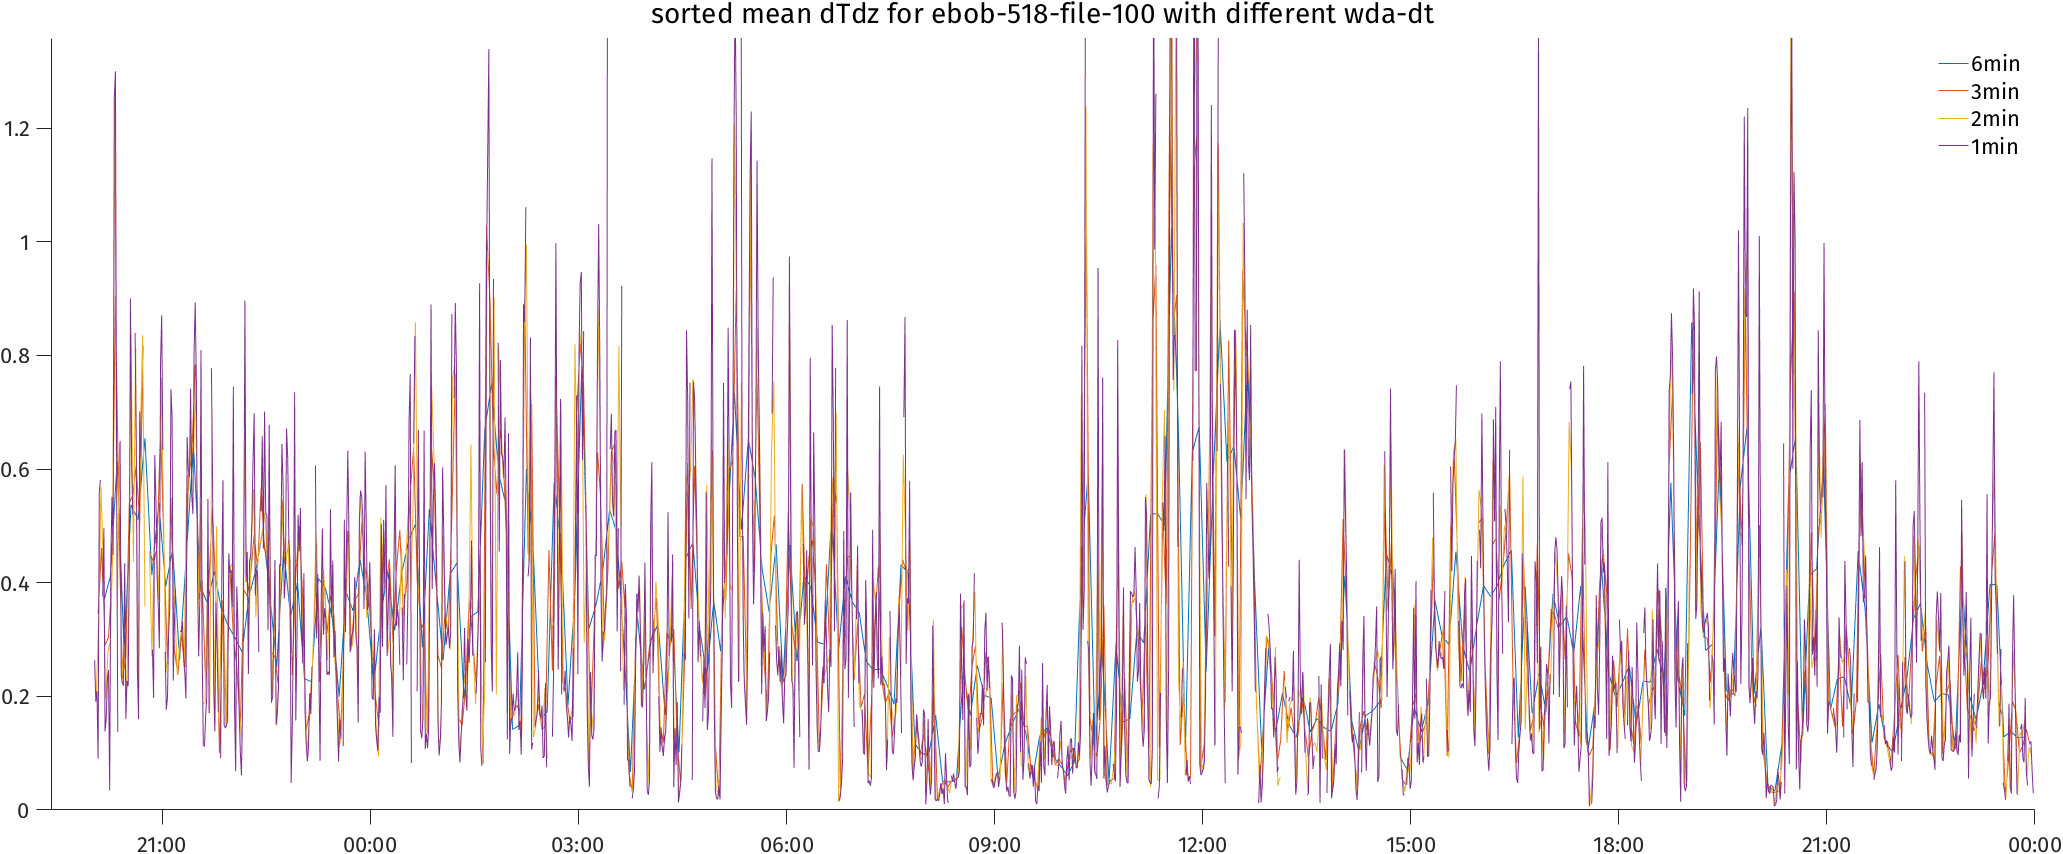
\includegraphics[width=0.9\textwidth]{figs/wda-sorted-dTdz-dt-variation.png}
  \caption{Variation of sorted mean gradient with time interval \texttt{wda\_dt}. Larger time intervals result in smoother gradient. This is for a time period with high stratification.}
  \label{fig:dTdz-dt}
\end{figure}

\subsection{Sign of vertical heat flux}
When salinity controls density, it is possible that $dT/dz < 0$ for extended periods of time.
Thorpe sorting cannot preserve this sign (unless there are coincident measurements of salinity, in which case you would sort density).
The only sensible thing to do is to determine the sign of the mean (or ``large-scale'') gradient from other sources such as nearby CTDs on the mooring, if available.
Currently \texttt{combine\_turbulence} uses the sign of the hourly running median of mooring $T_z$ (can be switched to internal $T_z$ using \texttt{CP.wda\_Tz\_sign}).
During times of low gradients ($T_z < $ \texttt{CP.min\_dTdz}), it uses the sign of the 2-hour running median since we want some sort of ``stable'' sign.

\subsection{Number of bins}

Currently the code uses 5 bins per minute of data and scales that according to \texttt{pflag.master.wda\_dt}. The nunmber of bins is set by setting \texttt{nquantiles} in \texttt{do\_wda\_estimate}. More bins mean better use of data but fewer $χ$ measurements to average in each bin. Few bins will result in the inability to determine gradients well because the temperature profiles could be too short to intersect 2 bin edges.

%%% Local Variables:
%%% mode: latex
%%% TeX-master: "docs"
%%% End:
